\section{DJ mix transcription}

In this section, we introduce a new application of NMF algorithm to
perform DJ mix transcription. We first study DJ hardware and software to
justify the transcription task as a matrix factorization problem, and
introduce the base Beta-NMF algorithm. We then show that the matrix
factorization can yield an intuitive representation of DJ mix
parameters. We propose a multi-pass extension of the NMF algorithm that
greatly improves its performance, and discuss additional modifications.
We then present example results and evaluate our method on a publicly
available dataset.

\subsection{DJ mixing hardware}

The DJs'' field of expression is defined by its hardware and/or
software: decks, mixing tables, and controllers. Despite the diversity
in brands and models, which offer varying feature sets, the underlying
workflow remains consistent across different setups. This consistency
allows us to generalize the signal path from recorded tracks to the
final mixed output, as depicted in
\hyperref[dj-signal-path]{{[}dj-signal-path{]}}.

\begin{figure}
\centering
\includesvg{dj-deck.svg}
\caption{Schematic view of the DJ mixing process}
\end{figure}

\phantomsection\label{dj-signal-path}{}

The signal path illustrated is directly derived from standard DJ setups,
encompassing both hardware and software environments.\footnote{It is
  noteworthy that DJ software is typically designed to emulate the
  functionality of traditional DJ hardware, thereby preserving the
  validity of this signal path.} The process can be described as
follows:

\begin{itemize}
\item
  Two or more DJ decks (in blue) are used as signal sources and play
  pre-recorded tracks and apply time-warping.
\item
  The signal from the decks is routed to the DJ mixer, which performs a
  weighted sum of the input signals. The mixer may also apply various
  effects, the most prevalent being a 3- or 4-band equalizer (EQ).
  Additional elements, such as external audio sources or audio effects,
  are also integrated at this stage.
\item
  Post-mixing, additional processing might be applied to the mixed
  output to meet specific distribution or venue requirements. This
  processing typically involves light modifications such as compression
  and equalization. However, given the minimal nature of these
  modifications, they will be considered negligible and thus omitted
  from further discussion in this report.
\end{itemize}

\subsection{Matrix representation of the DJ mixing process}

We now use this knowledge to introduce a matrix formulation of DJ
mixing, by considering a spectrogram reprensentation of the signals. We
achive this by grouping all non-time-based transformations, and modeling
any additional elements and timbral effects as additive noise, as
illustrated in \hyperref[separate-boxes]{{[}separate-boxes{]}}.

\begin{figure}
\centering
\includesvg{separate-boxes.svg}
\caption{Separated signal path}
\end{figure}

\phantomsection\label{separate-boxes}{}

Assuming the \(M\) constituting tracks of the mix are known, let
\(\forall i \in \lbrack 1\ldots M\rbrack\):

\begin{itemize}
\item
  \(\WW_{(i)}\) the spectrogram of track \(i\);
\item
  \(\HH_{(i)}\) the so-called \emph{activation matrix} of track
  \(i\), representing both the time-warping operations and the gain
  applied at the mixing stage;
\item
  \(\VV_{(i)} = \WW_{(i)}\HH_{(i)}\) the
  time-remapped spectrogram of track \(i\) with gain appplied;
\item
  \(\mathbf{\mathrm{N}}\) a noise matrix representing the timbral
  changes applied to the mix and/or tracks and any additional elements;
\item
  \(\mathbb{V}\) the spectrogram of the mix.
\end{itemize}

Using these notations, we can write:

\[\begin{aligned}
\VV & = \mathbf{\mathrm{N}} + \sum_{i = 1}^{M}\WW_{(i)}\HH_{(i)}
\end{aligned}\] \textless eq:mix\textgreater{}

An computation diagram of \hyperref[eq]{{[}eq{]}}:mix is given
\hyperref[nmf-djmix]{{[}nmf-djmix{]}}.

\begin{figure}
\centering
\includesvg{nmf-djmix.svg}
\caption{Matrix form of the DJ mixing process}
\end{figure}

\phantomsection\label{nmf-djmix}{}

Then, by defining two additional matrices \(\WW_{(a)}\) and
\(\HH_{(a)}\) of compatible dimensions so that
\(\mathbf{\mathrm{N}} = \WW_{(a)}\HH_{(a)}\), we can
rewrite \hyperref[eq]{{[}eq{]}}:mix as a simple matrix multiplication of
two large matrices by concatenation:

\[\begin{aligned}
\VV & = \WW_{(a)}\HH_{(a)} + \sum_{i = 1}^{M}\WW_{(i)}\HH_{(i)} \\
 & = \underset\WW{\underbrace{\begin{pmatrix}
\WW_{(1)}\WW_{(2)}\ldots\WW_{(M)}\WW_{(a)}
\end{pmatrix}}}\underset\HH{\underbrace{\begin{pmatrix}
\HH_{(1)} \\
\HH_{(2)} \\
 \vdots \\
\HH_{(M)} \\
\HH_{(a)}
\end{pmatrix}}}
\end{aligned}\] \textless eq:matmul\textgreater{}

Because we assume that the constituent tracks of the mix are known, the
(\(\WW_{(1)}\) to \(\WW_{(M)}\) submatrices are known.
Transcribing the DJ mix then amounts to determining the other
coefficients of \hyperref[eq]{{[}eq{]}}:matmul:

\begin{itemize}
\item
  If the noise matrix is assumed to be zero, estimating the gain and
  time-warping amounts to determining the coefficients of the
  \(\HH\) matrix while keeping the \(\XX\) matrix fixed.
\item
  If not, only part of the \(\XX\) matrix (\(\WW_{(1)}\)
  to \(\WW_{(M)}\) submatrices) is kept fixed, while the
  \(\WW_{(a)}\), \(\HH_{(1)}\) to
  \(\HH_{(M)}\) and \(\HH_{(a)}\) submatrices are
  estimated.
\end{itemize}

This can be understood as a matrix factorization problem. It is
well-suited to the NMF family of algorithms, which has proven especially
effective in audio source separation tasks, which we present in the next
section.

\subsection{NMF Algorithm}

\subsubsection{Beta-NMF and Multiplicative Update rules
\textless sec:beta-nmf\textgreater{}}

Let \(\WW \in {\mathbb{R}}_{+}^{F \times K}\),
\(\HH \in {\mathbb{R}}_{+}^{K \times N}\) and
\(\VV \in {\mathbb{R}}_{+}^{F \times N}\) non-negative
matrices. The NMF algorithm in its most basic form aims to minimise a
similarity measure \(\mathcal{D}\) between the \emph{target matrix}
\(\mathbb{V}\) and the \emph{estimated matrix}
\(\WW\HH\), and amounts to solving the following
optimization problem:

\[\min\limits_{\WW,\HH}\mathcal{D}\left( \VV~|~\WW\HH \right)\text{ with }\VV \geq 0,\WW \geq 0,\HH \geq 0\]
\textless eq:optimization-problem\textgreater{}

The similarity measure we use is the beta-divergence, which is defined
\(\forall\beta \in {\mathbb{R}}\) as follows:

\[\mathcal{D}_{\beta}\left. \left( \VV~|~\WW\HH \right) \right. = \sum_{f = 1}^{F}\sum_{n = 1}^{N}d_{\beta}\left. \left( \VV_{fn}~|~\left. (\WW\HH) \right._{fn} \right) \right.\]
\[d_{\beta}\left. \left( x~|~y \right) \right. = \begin{cases}
\frac{1}{\beta\left. (\beta - 1) \right.}\left. \left( x^{\beta} + \left. (\beta - 1) \right.y^{\beta} - \beta xy^{\beta - 1} \right) \right. & \text{ if }\beta \neq \left\{ 0,1 \right\} \\
x\ln\frac{x}{y} - x + y & \text{ if }\beta = 1 \\
\frac{x}{y} - \ln xy - 1 & \text{ if }\beta = 0
\end{cases}\] \textless eq:beta-divergence\textgreater{}

It can be noted that the beta-divergence is equivalent to:

\begin{itemize}
\item
  the Euclidian distance if \(\beta = 2\);
\item
  the Kullblack-Leibler divergence if \(\beta = 1\);
\item
  the Itakura-Saito divergence if \(\beta = 0\).
\end{itemize}

As shown in
\hyperref[fevotteNonnegativeMatrixFactorization2009]{{[}fevotteNonnegativeMatrixFactorization2009{]}}
and later extended in
\hyperref[fevotteAlgorithmsNonnegativeMatrix2011]{{[}fevotteAlgorithmsNonnegativeMatrix2011{]}},
an efficient and simple gradient descent algorithm for \(\XX\)
and \(\HH\) can be derived if the gradient of the divergence
w.r.t. a parameter \(\mathbf{\theta}\) is separable into its positive
and negative parts:

\[\delta_{\mathbf{\mathbf{\theta}}}\mathcal{D}_{\beta}\left( \VV~|~\WW\HH \right) = \delta_{\mathbf{\mathbf{\theta}}}^{+}\mathcal{D}_{\beta}\left( \VV~|~\WW\HH \right) - \delta_{\mathbf{\mathbf{\theta}}}^{-}\mathcal{D}_{\beta}\left( \VV~|~\WW\HH \right)\]
\textless eq:gradient-separation\textgreater{}

Using the notation trick described in
\hyperref[fevotteAlgorithmsNonnegativeMatrix2011]{{[}fevotteAlgorithmsNonnegativeMatrix2011{]}},
the so-called \emph{multiplicative update} rules can be
obtained\footnote{\(\odot\) and \(\frac{\ldots}{\ldots}\) stand
  respectively for Hadamard's (element-wise) product and division.}:
\[\mathbf{\theta} \leftarrow \mathbf{\theta} \odot \frac{\delta_{\mathbf{\mathbf{\theta}}}^{-}\mathcal{D}_{\beta}\left( \VV~|~\WW\HH \right)}{\delta_{\mathbf{\mathbf{\theta}}}^{+}\mathcal{D}_{\beta}\left( \VV~|~\WW\HH \right)}\]
\textless eq:mu-gradient\textgreater{}

With the beta-divergence, this yields the update rules of
\hyperref[algo]{{[}algo{]}}:mu-betadiv which can be efficiently
implemented, with strong monotonicity guarantees when
\(\beta \in \lbrack 0,2\rbrack\).

\begin{figure}
\centering
\begin{minipage}[t]{0.45\linewidth}
\end{minipage}
\hfill
\begin{minipage}[t]{0.45\linewidth}
\begin{enumerate}
\item
  \textbf{Initialize} \(\WW \geq 0\) and
  \(\HH \geq 0\)
\item
  \textbf{Until} convergence criterion is reached:

  \begin{enumerate}
  \item
    \(\HH \leftarrow \HH \odot \frac{\WW^{T}\left( (\WW\HH)^{\beta - 2} \odot \VV \right)}{\WW^{T}(\WW\HH)^{\beta - 1}}\)
  \item
    \(\WW \leftarrow \WW \odot \frac{\left( (\WW\HH)^{\beta - 2} \odot \VV \right)\HH^{T}}{(\WW\HH)^{\beta - 1}\HH^{T}}\)
  \end{enumerate}
\end{enumerate}
\end{minipage}
\caption{}
\end{figure}

\textless algo:mu-betadiv\textgreater{}

An interesting property of this algorithm is that any zeroes in
\(\HH\) or \(\XX\), by property of multiplication, remain
zero troughout the optimization process. We will exploit this property
in \hyperref[sec]{{[}sec{]}}:multi-pass.

More complex objective functions can be crafted by adding supplementary
functions to the similarity measure, for penalization or regularization
of the solutions. We detail the principle and some penalty functions
considered for DJ mix transcription in
\hyperref[sec]{{[}sec{]}}:penalty.

\subsubsection{Choosing the divergence and the type of spectrograms}

Previous research empirically shown that the Kullback-Leibler divergence
yields favorable results in source separation tasks when applied to
magnitude spectrograms
\hyperref[virtanenMonauralSoundSource2007]{{[}virtanenMonauralSoundSource2007{]}}.
Conversely, pairing the Itakura-Saito divergence with power spectrograms
has been shown to perform well, supported by a robust statistical model
\hyperref[fevotteMajorizationminimizationAlgorithmSmooth2011]{{[}fevotteMajorizationminimizationAlgorithmSmooth2011{]}}.

Additionally, {[}{]} explore the use of fractional values for the
parameter beta in source separation and suggests that spectrograms could
be raised to a fractional power. This approach is further refined by the
introduction of the tempered beta-divergence, where beta acts as a
temperature parameter that varies during the optimization process.
However, despite these theoretical advancements, we found no conclusive
evidence in the existing literature regarding the optimal approach for
our specific task.

Ultimately, after conducting our own experiments, we selected the
Itakura-Saito divergence applied to power spectrograms, as this
combination consistently produced the best results in our trials.

\subsection{Characterization of warp and gain transformations}

In this section, we present a model for time-warping and applying gain
to a signal within the spectral domain. We demonstrate that a specific
solution for the activation matrix exists, which reveals intuitive
structural properties. Following this, we define estimators for both
gain and time-warping, and conduct an analysis of their robustness in
the presence of noise and other sources of uncertainty.

\subsubsection{The ideal kernel}

Let \(x\lbrack t\rbrack\) be a real-valued signal, and define the
following:

\begin{itemize}
\item
  \(f:\tau \mapsto t\) a time-warping injective function that maps a mix
  time step \(\tau\) to a track time step \(t\);
\item
  \(g\lbrack\tau\rbrack\) a gain factor sequence;
\item
  \(y\lbrack\tau\rbrack\) the time-warped (by \(f\)) and gain-modulated
  (by \(g\)) transformation of \(x\);
\item
  \(w\) an arbitrary window function of length \(M\).
\end{itemize}

We define \({\mathbb{X}} = \left( {\mathbb{X}}_{mt} \right)\) as the
spectrogram matrix of \(x\) (\(M\) frequency bins \(\times T\) time
steps):
\[{\mathbb{X}}_{mt} = \left| {\sum_{n = 1}^{M}x\lbrack n + t\rbrack w\lbrack n\rbrack e^{- j2\pi n\frac{m}{M}}} \right|^{2}\]
\textless eq:stft\textgreater{}

Similarly, we define
\({\mathbb{Y}} = \left( {\mathbb{Y}}_{m\tau} \right)\) as the power
spectrogram matrix of \(y\) (\(M\) frequency bins \(\times K\) time
steps). We show that \(\mathbb{Y}\) can be expressed in terms of
\(\mathbb{X}\) as follows:

\[\begin{aligned}
{\mathbb{Y}}_{m\tau} & = \left| {g\lbrack\tau\rbrack\sum_{n = 1}^{M}x\left\lbrack n + f\lbrack\tau\rbrack \right\rbrack w\lbrack n\rbrack e^{- j2\pi n\frac{m}{M}}} \right|^{2} \\
 & = g\lbrack\tau\rbrack^{2}{\mathbb{X}}_{m,f\lbrack\tau\rbrack}
\end{aligned}\] \phantomsection\label{xy-relation}{}

We can then find a matrix
\(\HH = \left( \HH_{t\tau} \right)\) (of dimensions
\(T\) time steps \(\times K\) time steps) that satisfies:
\[\begin{aligned}
{\mathbb{Y}} & = {\mathbb{X}}\HH \Leftrightarrow {\mathbb{Y}}_{m\tau} = \sum_{t = 0}^{T - 1}{\mathbb{X}}_{mt}\HH_{t\tau}
\end{aligned}\] \phantomsection\label{matmul}{}

The \emph{ideal kernel} \(\HH^{\text{ideal}}\), a solution to
\hyperref[matmul]{{[}matmul{]}}, is of particular interest. When viewed
as an image, this matrix offers an intuitive understanding of the
transformations applied to \(x\lbrack t\rbrack\), as illustrated in
\hyperref[fig]{{[}fig{]}}:time-time.

The ideal kernel is defined as:

\[{\HH^{\text{ideal}}}_{t\tau} ≝ g\lbrack\tau\rbrack^{2}\delta_{t,f\lbrack\tau\rbrack}\]
\phantomsection\label{ideal-kernel}{} where \(\delta_{a,b}\) is the
Kronecker delta function, defined by \(\delta_{a,b} = \begin{cases}
1\text{ if }a = b \\
0\text{ otherwise}
\end{cases}\).

\begin{figure}
\centering
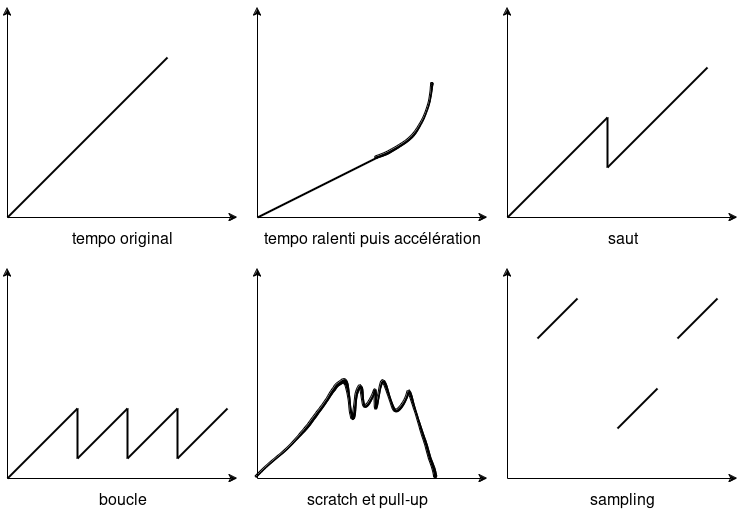
\includegraphics{../2024-03-26/temps-temps.drawio.png}
\caption{Some examples of the structures emerging in
\(\HH^{\text{ideal}}\), with the associated DJ nomenclature.}
\end{figure}

\textless fig:time-time\textgreater{}

\subsubsection{Estimation of the warp and gain values}

We define the following estimators for the gain and time-warping
functions:

\[\overset{\sim}{g}\lbrack\tau\rbrack = \sqrt{\sum_{t = 1}^{T}\HH_{t\tau}}\]
\phantomsection\label{gain_estimator_sum}{}
\[\overset{\sim}{f}\lbrack\tau\rbrack = \text{ argmax}_{t \in \lbrack 1\ldots T\rbrack}\HH_{t\tau}\]
\phantomsection\label{time_estimator_argmax}{}

Intuitively, \(\overset{\sim}{g}\lbrack\tau\rbrack\) represents the
energy of a column of \(\HH\), while
\(\overset{\sim}{f}\lbrack\tau\rbrack\) corresponds to the position of
its peak.

In the case of the ideal kernel
(\hyperref[ideal-kernel]{{[}ideal-kernel{]}}), it can be easily shown
that \(\overset{\sim}{f}\) and \(\overset{\sim}{g}\) are exact
estimators, meaning they perfectly recover the gain and time-warping
functions. However, in practical scenarios, the optimization algorithm
used to compute \(\HH\) does not inherently guarantee convergence
to this ideal solution.

In practice, the NMF tends to converge towards the similarity matrix
between \(y\) and \(x\), rather than the idealized sparse solution with
line features. This underscores the need to incorporate additional
techniques that guide the algorithm towards convergence to the ideal
solution, thereby ensuring that the estimators remain robust in the
presence of noise and other uncertainties. We discuss briefly a few
examples of such indeterminacies in the next section.

\subsubsection{Sources of indeterminate forms}

\paragraph{Impact of self-similar input signals}

\begin{figure}
\centering
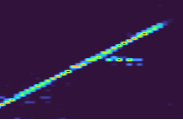
\includegraphics{../2024-05-30/longue-note.png}
\caption{Artifacts in \(\HH\) caused by spectrally similar
frames.}
\end{figure}

\textless fig:indeterminacies\textgreater{}

\begin{figure}
\centering
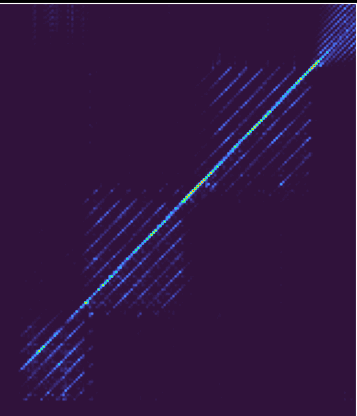
\includegraphics{../2024-05-17/image-2.png}
\caption{Parallel line structures in \(\HH\) caused by loops in
the reference tracks.}
\end{figure}

\textless fig:parallel-lines\textgreater{}

Given the nature of musical signals, two columns of \(\mathbb{X}\) could
be almost identical (\hyperref[fig]{{[}fig{]}}:parallel-lines), for
example in the presence of a loop in electronic music
(\hyperref[fig]{{[}fig{]}}:indeterminacies).

Let \(t_{1}\) and \(t_{2}\) be the time steps at which this is true, and
\(\tau_{1} = f^{- 1}\left\lbrack t_{1} \right\rbrack\) and
\(\tau_{2} = f^{- 1}\left\lbrack t_{2} \right\rbrack\) their
antecedents. We then have \(\forall m\):
\[{\mathbb{Y}}_{m\tau_{1}} = {\mathbb{Y}}_{m\tau_{2}} = g\left\lbrack \tau_{1} \right\rbrack^{2}{\mathbb{X}}_{mt_{1}} = g\left\lbrack \tau_{2} \right\rbrack^{2}{\mathbb{X}}_{mt_{2}}\]

Visually, this corresponds to multiple activations per column of
\(\HH\), with the energy of the activations being distributed
arbitrarily between four points:
\(\left\{ \left( t_{1},\tau_{1} \right),\left( t_{1},\tau_{2} \right),\left( t_{2},\tau_{1} \right),\left( t_{2},\tau_{2} \right) \right\}\).
Fortunately, such indeterminacies do not invalidate
\(\overset{\sim}{g}\), but the same can not be said of
\(\overset{\sim}{f}\).

\paragraph{Impact of hop size discretization}

Usually, the spectrogram is not computed for every sample of a signal as
in our earlier definition (\hyperref[eq]{{[}eq{]}}:stft), but at
uniformly sampled time instants spaced by a \emph{hop size} \(h\). This
effectively downsamples the time steps to \(\underset{¯}{t} = ht\) and
\(\underset{¯}{\tau} = h\tau\), leading to the following expressions for
the spectrograms:

\[{\mathbb{X}}_{m\underset{¯}{t}} = \left| {\sum_{n = 0}^{M - 1}x\lbrack n + ht\rbrack w\lbrack n\rbrack e^{- j2\pi n\frac{m}{M}}} \right|^{2}\]
\[\begin{aligned}
{\mathbb{Y}}_{m\underset{¯}{\tau}} & = \left| {g\lbrack\tau\rbrack\sum_{n = 0}^{M - 1}x\left\lbrack n + f\lbrack h\tau\rbrack \right\rbrack w\lbrack n\rbrack e^{- j2\pi n\frac{m}{M}}} \right|^{2}
\end{aligned}\]

Due to this discretization, there may not be an exact alignment between
\(\underset{¯}{t}\) and \(\underset{¯}{\tau}\). Consequently, the
activations within \(\HH\) could be distributed across
neighboring cells.

\subsection{The Multi-pass NMF Algorithm
\textless sec:multi-pass\textgreater{}}

DJ mixes consist of multiple tracks, each typically appearing only
within a specific segment of the mix. Consequently, the activation
matrix \(\HH\) is expected to exhibit block-sparsity, as depicted
in \hyperref[fig]{{[}fig{]}}:block-sparse.

\begin{figure}
\centering
\includesvg[width=0.8\textwidth,height=\textheight]{block-sparse.svg}
\caption{Expected block-sparse form of the activation matrix in a
5-track mix, with transition regions annotated.}
\end{figure}

\textless fig:block-sparse\textgreater{}

While applying NMF directly to spectrograms computed with the desired
hop size may yield the expected results, our experiments suggest that an
increased number of tracks and smaller window sizes exacerbate
cross-track indeterminacies. This issue arises especially because tracks
in a mix are often stylistically or tonally similar.

To address this we propose a multi-pass NMF algorithm, described in
\hyperref[fig]{{[}fig{]}}:multipass-flow, paired with a
filter-threshold-resize procedure inbetween each pass.

The methodology involves initially performing NMF on spectrograms
computed with a significantly large hop size (on the order of minutes)
to obtain the approximate position of each track in the mix. The
resultant activation matrix is then processed through filtering to
reduce noise, followed by blurring and thresholding. This matrix is
resized to match the dimensions corresponding to the next smaller hop
size, resulting in a larger activation matrix that serves as the
initialization for the subsequent NMF pass. This iterative process
continues until the desired hop size is reached.

\begin{figure}
\centering
\includesvg[width=0.5\textwidth,height=\textheight]{multipass-flowchart.svg}
\caption{Flow chart of the multipass NMF algorithm}
\end{figure}

\textless fig:multipass-flow\textgreater{}

By property of the NMF with multiplicative updates, regions of the
matrix set to zero during thresholding will remain zero in subsequent
iterations, thereby avoiding spurious activations. However, careful
selection of filtering and thresholding techniques is crucial to avoid
the inadvertent elimination of valid activations.

Moreover, when coupled with an appropriate block-sparse matrix
representation, this approach significantly enhances processing
efficiency and memory usage, which is particularly advantageous given
the large size of spectrogram matrices at smaller hop sizes.

As an illustration, we ran the multipass NMF algorithm on a 3-track mix
with gradually decreasing hop sizes. The
\hyperref[fig]{{[}fig{]}}:multipass depicts the estimated activation
matrices at the end of each pass. The first hop size (15 seconds) gives
a rough estimation of the positions of the constituent tracks in the
mix. and with each subsequent pass, the activation matrices are larger
the activations more precise, and become less noisy and more sparse.

\begin{figure}
\centering
\includesvg[width=1.2\textwidth,height=\textheight]{multipass.svg}
\caption{Vizualization of successive estimated activation matrices
during execution of the multipass NMF algorithm. Zero-valued cells are
depicted in white.}
\end{figure}

\textless fig:multipass\textgreater{}

\subsubsection{Filter-threshold-resize procedure}

The filter-threshold-resize procedure is integral to the effectiveness
of the multipass NMF algorithm. The steps of the procedure are described
below, and illustrated \hyperref[fig]{{[}fig{]}}:interpass.

\begin{description}
\item[Morpohological filtering]
A line-enhancing filter is applied on each submatrix
\(\HH_{(i)}\) of \(\HH\), inspired by {[}{]}. This
filter is designed using fixed-length one-pixel-wide straight line
kernels with slopes distributed between a minimum and maximum value. A
morphological opening operation is performed on \(\HH\) with
these kernels, and the results are aggregated. This process eliminates
activations shorter than the specified length and that do not meet the
expected slope limits, effectively denoising the activation matrix.
\item[Blurring]
A gaussian blur is applied on each submatrix with a small kernel. This
has the effect of smearing the activations in time.
\item[Thresholding]
Set activations below a specified threshold to zero.
\item[Resizing]
The thresholded activation matrix is then resized to a larger size, i.e.
corresponding to a smaller hop size, and returned.
\end{description}

\begin{figure}
\centering
\includesvg[width=1.5\textwidth,height=\textheight]{interpass.svg}
\caption{Vizualisation of the steps of the filter-threshold-resize
procedure on a 3-track mix. The input activation matrix corresponds to a
hop size of 3 seconds, and the output corresponds to a hop size of 1
second. Zero-valued cells are depicted in white.}
\end{figure}

\textless fig:interpass\textgreater{}

\subsection{Downsampling and use of the mel transform}

DJ mixes are typically lengthy, ranging from 30 minutes to several
hours, and as they consist of musical signals, their frequency bandwidth
is notably extensive. When employing the Short-Time Fourier Transform
(STFT) with standard hop durations and a typical number of frequency
bins for musical signals, the resulting feature matrix can become
exceedingly large. This leads to substantial memory usage and elevated
resource consumption.

In order to mitigate these issues, we have opted to use relatively large
hop durations. This approach not only reduces the computational load but
also offers an additional advantage: longer hop durations are better
adapted to the temporal structures inherent in music. The hop duration
however is not fixed, as is explained in
\hyperref[sec]{{[}sec{]}}:multi-pass.

Additionally, we compress the frequency information using the mel-scale
transform
\hyperref[stevensScaleMeasurementPsychological1937]{{[}stevensScaleMeasurementPsychological1937{]}}.
This transform groups nearby frequencies into bins based on a perceptual
model of human hearing, which is particularly well-suited for processing
musical signals. Importantly, this transform has no effect on the ideal
kernel and our estimators.

Let \(\mathbf{M}\) be a matrix of mel filterbank coefficients. The
mel-spectrograms are calculated from the regular spectrograms:
\({\mathbb{X}}^{\text{mel }} = \mathbf{M}{\mathbb{X}}\) and
\({\mathbb{Y}}^{\text{mel }} = \mathbf{M}{\mathbb{Y}}\). Then we have:
\[\begin{aligned}
{{\mathbb{Y}}^{\text{mel}}}_{m\tau} & = \sum_{i}\mathbf{M}_{mi}{\mathbb{Y}}_{i\tau} \\
 & = g\lbrack\tau\rbrack^{2}\sum_{i}\mathbf{M}_{mi}{\mathbb{X}}_{i,f\lbrack\tau\rbrack} \\
 & = g\lbrack\tau\rbrack^{2}{{\mathbb{X}}^{\text{mel}}}_{m,f\lbrack\tau\rbrack}
\end{aligned}\]

So the ideal kernel \(\HH^{\text{ideal}}\) is still clearly a
solution of \hyperref[matmul]{{[}matmul{]}}.

\subsection{Analysis window overlap}

A key parameter when working with spectrograms is the overlap factor of
the analysis windows. In order to emphasize the temporal continuity of
the musical signals, we use high overlap factors: our experiments have
shown that a window size of 6 to 8 times the hop size give the best
results. It has experimentally shown to be highly effective in reducing
indeterminacies, but tends to smooth out the results as a side-effect,
which can potentially obscure finer details in the signal, as shown in
\hyperref[fig]{{[}fig{]}}:overlap.

Typically, such large window sizes would result in a substantial
increase in the number of frequency bins, leading to higher
computational demands. However, by applying the mel-scale transform, we
effectively mitigate this issue.

\begin{longtable}[]{@{}lll@{}}
\caption{Comparison of the influence of different overlap factors. Top
row: estimated activation matrices. Bottom row: zooms on the middle
activation.}\tabularnewline
\toprule\noalign{}
\endfirsthead
\endhead
\bottomrule\noalign{}
\endlastfoot
\includesvg{overlap-1.svg} & \includesvg{overlap-8.svg} &
\includesvg{overlap-16.svg} \\
\end{longtable}

\textless fig:overlap\textgreater{}

\subsection{Spectrogram normalization}

To improve the numeric stability of the NMF, the columns of
\(\mathbb{X}\) are typically normalized to sum to 1. We also normalize
\(\mathbb{Y}\) by a single factor\footnote{Normalizing by column as for
  \(\mathbb{X}\) would cancel out the gain information in
  \(\HH\).}. We show that this results in a simple scaling factor
for \(\HH\) and therefore for the estimators.

Let the scaling factors \(\mathbf{k}_{t} ≝ \sum_{i}{\mathbb{X}}_{it}\)
and \(\kappa ≝ \sum_{i}\sum_{t}{\mathbb{Y}}_{it}\).

The normalized spectrograms are:
\[{{\mathbb{X}}^{\text{norm}}}_{mt} ≝ \frac{{\mathbb{X}}_{mt}}{\mathbf{k}_{t}}\]

\[{\mathbb{Y}}^{\text{norm }} ≝ \frac{\mathbb{Y}}{\kappa}\]

Using \hyperref[xy-relation]{{[}xy-relation{]}}:
\[{{\mathbb{Y}}^{\text{norm}}}_{m\tau} = \frac{\mathbf{k}_{t}}{\kappa}g\lbrack\tau\rbrack^{2}{{\mathbb{X}}^{\text{norm}}}_{m,f\lbrack\tau\rbrack}\]

We can then deduce the ideal normalized kernel
\(\HH^{\text{norm}}\) as a solution to
\hyperref[matmul]{{[}matmul{]}}:

\[\begin{aligned}
{\HH^{\text{norm}}}_{t\tau} & ≝ \frac{\mathbf{k}_{t}}{\kappa}g\lbrack\tau\rbrack^{2}\delta_{t,f\lbrack\tau\rbrack} \\
 & = \frac{\mathbf{k}_{t}}{\kappa}{\HH^{\text{ideal}}}_{t\tau}
\end{aligned}\]

\subsection{Thresholding of low-power frames}

Recorded music tracks often contain moments of silence or faint noise at
the beginning and end of the signal. It is also quite common to find
fade-out endings at the end of tracks, or reverberation tails. These
elements appear as low-power frames in the feature matrices.
Reverberation tails, in particular, are problematic due to their
spectral similarity to the rest of the track, which can introduce
indeterminacies in the analysis.

Additionally, low-power frames are unlikely to be present in a DJ mix,
as DJs typically focus on playing the most musically significant
portions of tracks, omitting the very beginning and end.

To address this, we detect and mark low-power frames in the input track
spectrograms as unused and set the corresponding cells in the activation
matrix to zero, effectively preventing these frames from contributing to
the optimization process.

\subsection{Implementation}

The algorithm has been implemented in Python. By leveraging the
pytorch\footnote{\url{https://pytorch.org}} framework, the optimization
process can run on both CPU and GPU and benefit from parallel matrix
multiplications on the latter.

We summarize the tunable parameters in
\hyperref[table]{{[}table{]}}:hyperparams along with their typical
values. These can be further adjusted with prior knowledge of the
mixes'' characteristics.

\begin{longtable}[]{@{}
  >{\raggedright\arraybackslash}p{(\columnwidth - 6\tabcolsep) * \real{0.2500}}
  >{\raggedright\arraybackslash}p{(\columnwidth - 6\tabcolsep) * \real{0.2500}}
  >{\raggedright\arraybackslash}p{(\columnwidth - 6\tabcolsep) * \real{0.2500}}
  >{\raggedright\arraybackslash}p{(\columnwidth - 6\tabcolsep) * \real{0.2500}}@{}}
\caption{Summary of tunable parameters}\tabularnewline
\toprule\noalign{}
\endfirsthead
\endhead
\bottomrule\noalign{}
\endlastfoot
\textbf{Name} & \textbf{Description} & \textbf{Unit} & \textbf{Typical
value} \\
\texttt{FS} & Sampling rate & Hz & 22050 \\
\texttt{HOP\_SIZES} & Decreasing list of hop durations & s. &
\texttt{{[}20,\ 10,\ 2,\ 0.5,\ 0.1{]}} \\
\texttt{OVERLAP} & STFT analysis window overlap factor & \begin{itemize}
\tightlist
\item
\end{itemize} & 6 to 8 \\
\texttt{NMELS} & Number of mel bands & \begin{itemize}
\tightlist
\item
\end{itemize} & 64 to 256 \\
\texttt{SPEC\_POWER} & STFT power & \begin{itemize}
\tightlist
\item
\end{itemize} & 2 \\
\texttt{DIVERGENCE} & Divergence function & \begin{itemize}
\tightlist
\item
\end{itemize} & \(\mathcal{D}_{\beta}\) with \(\beta = 0\) \\
\texttt{LOW\_POWER\_THRESHOLD} & Threshold under which frames from input
tracks are discarded & dB & -40 \\
\texttt{CARVE\_THRESHOLD} & Threshold under which a cell of the
activation matrix is deemed zero & dB & -120 \\
\texttt{CARVE\_BLUR\_SIZE} & Size of the gaussian blur kernel &
\begin{itemize}
\tightlist
\item
\end{itemize} & 3 \\
\texttt{CARVE\_MIN\_DURATION} & Minimum line duration for morphological
filtering & s. & 10 \\
\texttt{CARVE\_MAX\_SLOPE} & Maximum allowed deviation from original
playing speed & ± \% & 10 to 50 \\
\texttt{NOISE\_DIM} & Number of columns for noise estimation &
\begin{itemize}
\tightlist
\item
\end{itemize} & 0 to 50 \\
\end{longtable}

\textless table:hyperparams\textgreater{}

\subsection{Example results}

We run the algorithm on several constructed mixes, that showcase mix
scenarios with the typical transformations that we aim to be able to
reverse engineer. All figures depict:

\begin{itemize}
\item
  On the left, the final estimated activation matrix, with zero-valued
  cells in gray;
\item
  In the middle, the estimated gain (dots) and ground truth (dashed)
\item
  On the right, the estimated warp function (dots) and ground truth
  (dashed).
\end{itemize}

Firstly, we focus on time transformations using ``mixes'' composed of a
single track. The \hyperref[fig]{{[}fig{]}}:jumploop presents a single
track that has been sliced and looped, and the
\hyperref[fig]{{[}fig{]}}:timestretch corresponds to a single track that
has been time-stretched by the use of the Rubberband\footnote{\url{https://breakfastquay.com/rubberband/}}
library. Although presenting some artifacts, especially in the gain
estimation for the timestretched track, we can see that the time-warping
function is estimated accurately.

\begin{figure}
\centering
\includesvg[width=1.4\textwidth,height=\textheight]{jumploop.svg}
\caption{Results for a sliced track with loops and jumps.}
\end{figure}

\textless fig:jumploop\textgreater{}

\begin{figure}
\centering
\includesvg[width=1.4\textwidth,height=\textheight]{timestretch.svg}
\caption{Results for a time-stretched track.}
\end{figure}

\textless fig:timestretch\textgreater{}

Secondly, we focus on overlapping tracks. The
\hyperref[fig]{{[}fig{]}}:linear-mix depicts a simple mix of two tracks
with a large transition region composed of a crossfade. Despite having
no kwowledge of the form of cross-fading used, the method correctly
estimates the gain for both tracks, and mostly correctly estimates the
warp function.

It should be noted that the figure depict the raw warp function
estimations, which is computed for all tracks for the whole duration of
the mix. Hence, the points outside of the tracks'' playing range are
effectively noise and could be filtered, for example, using a simple
threshold on the gain estimation.

\begin{figure}
\centering
\includesvg[width=1.4\textwidth,height=\textheight]{linear-mix.svg}
\caption{Beat-synchronous mix of two tracks with linear fades.}
\end{figure}

\textless fig:linear-mix\textgreater{}
